% 環境設定関連 %
\documentclass[a4paper, 12pt]{ltjsarticle}
\usepackage{type1cm}
\usepackage{luatexja}
\usepackage{amsmath}
\usepackage{array}
\usepackage{bm}
\usepackage{cite}
\usepackage{graphicx}
\usepackage{mathrsfs}
\renewcommand{\footnotesize}{\small}

%\usepackage[utf8]{inputenc}
\bibliographystyle{junsrt}
\usepackage[top=35truemm, bottom=30truemm,left=30truemm,right=30truemm]{geometry}
% 横方向の文字数を４０文字にするには、27truemmに設定する必要がある。%

% ヘッダーの設定 %
\usepackage{fancyhdr}
\pagestyle{fancy}
\lhead{} %ヘッダーの左側に書くやつ（ここにプリントタイトル入れるのがオススメ）
\chead{} %ヘッダーの中央に書くやつ
%\rhead{第\thechapter 章 \thesection 節} %ヘッダーの右側に書くやつ
\lfoot{} %フッターの左側に書くやつ
\cfoot{\thepage} %フッターの中央に書くやつ（ここに\thepageを入れるとページ数を表示）
\rfoot{} %フッターの右側に書くやつ

\usepackage[pdfencoding=auto]{hyperref}
\hypersetup{% hyperrefオプションリスト
setpagesize=false,
 bookmarksnumbered=true,
 bookmarksopen=true,
 colorlinks=true,
 linkcolor=blue,
 citecolor=blue,
}

\title{日本語版Lua\LaTeX テンプレート}
\author{著者}
\date{yyyy年mm月dd日}

\begin{document}
\maketitle

\section{template}
	Template is here.
	Reference is \cite{AAAA}.
	
	\begin{itemize}
		\item 日本語版のLuaLatex用テンプレートです（但しarticle用）
		\item 参考文献は、bibtex を用いております。
	\end{itemize}
	\subsection{bibtexを含めたコンパイル方法}
	\begin{itemize}
		\item  bibtexのコンパイルは、
			\begin{enumerate}
				\item Lualatexのコンパイル
				\item pbibtex のコンパイル
				\item Lualatexのコンパイル
				\item Lualatexのコンパイル
			\end{enumerate}
		 の4段階で行う必要があります。
	 \end{itemize}
	
	\begin{figure}[!htbp]
		\begin{center}
			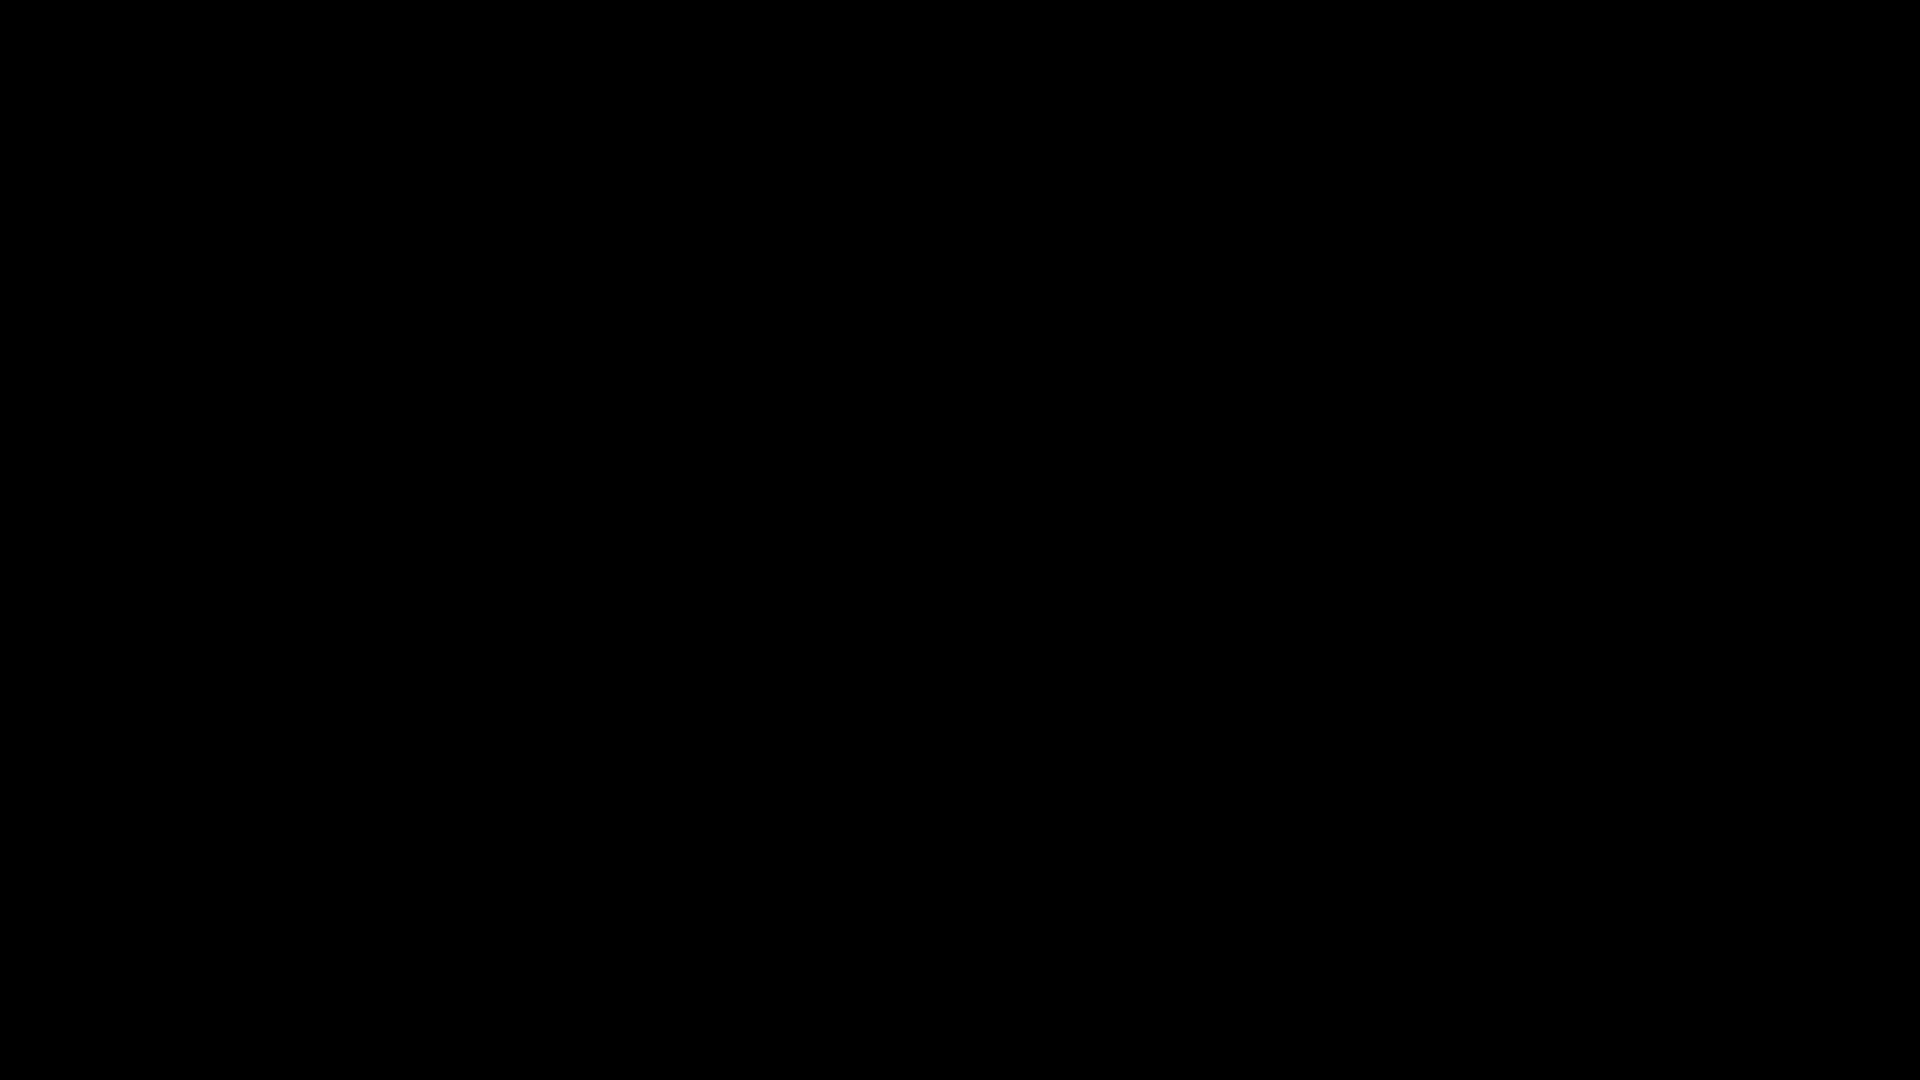
\includegraphics[width=10.0cm]{./fig/fig1.png}
			\caption{テスト画像}
			\label{fig:fig1}
		\end{center}
	\end{figure}
	
	図はfigフォルダを作成して、挿入するようにしております（図\ref{fig:fig1}参照)。

\bibliography{./ref/reference.bib}
\end{document}
